\documentclass[10pt,a4paper]{article}
\usepackage{amsmath,amssymb,amsthm,graphicx}
\usepackage{tikz}
\usepackage{amssymb,amsmath,amsthm}
\usepackage{enumitem}
\usepackage[dvipsnames]{xcolor}
\newcounter{propcounter}
\usepackage{graphicx}
\usepackage{ifthen,latexsym,fixmath}
\newcommand\norm[1]{\left\lVert#1\right\rVert}
\newcommand\innerp[1]{\langle #1 \rangle}
\newcommand\innerpbig[1]{\Big\langle #1 \Big\rangle}

\newenvironment{poc}{\begin{proof}[Proof of claim]\renewcommand*{\qedsymbol}{$\blacksquare$}}{\end{proof}}

\newcommand{\V}[1]{\mathbold{#1}}
\newtheorem{theorem}{Theorem}[section]
\newtheorem{lemma}[theorem]{Lemma}
\newtheorem{observation}[theorem]{Observation}
\newtheorem{proposition}[theorem]{Proposition}
\newtheorem{corollary}[theorem]{Corollary}
\newtheorem{claim}[theorem]{Claim}
\newtheorem{conjecture}[theorem]{Conjecture}
\newtheorem{problem}[theorem]{Problem}
\newtheorem{fact}[theorem]{Fact}
\newtheorem{conjx}{Conjecture}
\newtheorem{probx}[conjx]{Problem}
\renewcommand{\theconjx}{\Alph{conjx}}%"letter-numbered" theorems
\theoremstyle{definition}
\newtheorem{remark}[theorem]{Remark}
\newtheorem{definition}[theorem]{Definition}
\def\al{{\alpha}}
\def\de{{\delta}}
\def\eps{{\varepsilon}}

\newcommand{\iminnerp}[1]{{\rm{Im}}\langle #1 \rangle}
\newcommand{\reinnerp}[1]{{\rm{Re}}\langle #1 \rangle}
\newcommand{\im}[1]{{\rm{Im}}(#1)}
\newcommand{\re}[1]{{\rm{Re}}(#1)}
\newcommand{\diam}[1]{{\rm{diam}}(#1)}
\newcommand{\height}[1]{{\rm{height}}(#1)}
\newcommand{\mbf}[1]{\mathbf{#1}}
\newcommand{\ceil}[1]{\lceil{#1}\rceil}
\newcommand{\floor}[1]{\lfloor{#1}\rfloor}
\newcommand{\ex}{\mathbb{E}}
\newcommand{\eul}{e}
\newcommand{\pr}{\mathbb{P}}
%\newcommand{\RT}{\mathbb{RT}}
\newcommand{\sS}{\mathsf{S}}
\newcommand{\sN}{\mathbb{N}}
\newcommand{\sC}{\mathbb{C}}
\newcommand{\sR}{\mathbb{R}}
\newcommand{\sZ}{\mathbb{Z}}
\newcommand{\slice}{\mathsf{slice}}
\newcommand{\rt}{{\mathsf{RT}}}


\newcommand*{\abs}[1]{\lvert#1\rvert}
\newcommand*{\bigabs}[1]{\bigl|#1\bigr|}
\newcommand*{\Bigabs}[1]{\Bigl|#1\Bigr|}
\title{Complex Bollobas-Erdos graphs with arbitrary rational cross density}
\author{Hong Liu, Christian Reiher, Maryam Sharifzadeh, Katherine Staden}
\date{arxiv:2103.10423v2; CC BY 4.0}
\begin{document}
\maketitle
\noindent\textit{Editorial note.} The printed bound at source964 is too strong for odd p: an open half-plane through0 contains at most ceil(p/2) p-th roots. The actual assumed clique at958 already gives |X|>=ceil((p+ell+1)/2)>ceil(p/2), because ell>=1, so the author convex-hull contradiction still follows. The printed line is retained; it is not asserted literally true for odd p.\par\medskip
\noindent\textit{Editorial note.} In the rotation label set at962 the base vertex x0 has label0; its distance to rho\textasciicircum{}0*x0 is0. Every other vertex of X has a unique nonzero label by the root-separation lemma. This is a convention for the label set, not a loop edge added to the graph.\par\medskip
\noindent\textit{Editorial note.} The far-pair auxiliary statement948-949 needs a clique with at least2 vertices. Its only application in the counted proof is to Y, where959 gives |Y|>=ell+1>=2. The unrestricted auxiliary statement is not counted as a separate result.\par\medskip
\noindent\textit{Editorial note.} At939 the authors explicitly omit the upper-degree calculation. The independent reviews confirm that the already proved mu/4 cell perturbation and angle estimate925-937 apply in reverse to place neighboring cells inside a slightly enlarged phase interval, whose uniform phase measure gives the stated bound. The omission is disclosed; no generated calculation is presented as author proof.\par\medskip
\noindent\textit{Editorial scope.} Count only GBE. All construction and local verification text is retained. Quantitative cap/partition results are explicit standard inputs; source-local rotation and mixed-clique arguments are included as full author text.\par\medskip
\noindent\textit{Allowed standard prerequisites (editorial).}\begin{itemize}
\item Spherical cap measure bounds and equal-measure small-diameter partitions. The explicit stated quantitative bounds are allowed inputs. They do not give the phase-window graph, clique exclusion or prescribed rational density.
\item Spherical isoperimetry and Caratheodory theorem in the plane. Translate cap bounds to two-set separation; represent zero in a convex hull by at most three roots of unity.
\item Hierarchy of asymptotic parameters. Choose K, epsilon and k in the stated order, then choose n sufficiently large; use diagonal choice to turn the displayed quantitative errors into little-o bounds.
\end{itemize}\medskip
Ramsey graphs for cliques are believed to be random-like; while on the other hand, the Tur\'an graphs from extremal graph theory are highly structured. Initiated in 1969 by S\'os, and later generalised by Erd\H{o}s, Hajnal, S\'os and Szemer\'edi~\cite{EHSSz}, \emph{Ramsey-Tur\'an theory} combines flavours of graph Ramsey and Tur\'an problems. The \emph{Ramsey-Tur\'an number} $\rt_p(n,K_q,m)$ is the maximum number of edges in an $n$-vertex $K_q$-free graph $G$ with $\alpha_p(G)\le m$, where $\al_p(G)=\max\{|U|:U\subseteq V(G)\text{ and }G[U]\text{ is }K_p\text{-free}\}$ is the \emph{$p$-independence number} of $G$. Notice that when $p=2$ and $m=n$, we recover the Tur\'an number of $K_q$; and as we consider large graphs, that is $n\rightarrow\infty$, by Ramsey's theorem, $m$ should be taken as a function of $n$.

The classical setting of sublinear independence number is defined as follows. Let $\varrho_p(q)$ be the \emph{Ramsey-Tur\'an density}: 
$$
\varrho_p(q) := \lim_{\eps\rightarrow 0}\lim_{n\rightarrow \infty}\frac{\rt_p(n,K_q,\eps n)}{\binom{n}{2}}.
$$
The existence of the limit was shown by Erd\H{o}s, Hajnal, Simonovits, S\'os and Szemer\'edi~\cite{EHSSSz}. Then $\rt_p(n,K_q,o(n)):=\varrho_p(q){n\choose 2}+o(n^2)$.

\begin{conjx}[\cite{EHSSSz}, Conjecture~2.9]\label{conj}
	The asymptotic extremal graphs $G$ for $\varrho_p(q)$ have the following structure.
	Let $q=pt+r+2$ where $t\in\mathbb{N}$ and $0 \leq r < p$. Then there is a partition $V(G)= V_0\cup V_1 \cup \ldots \cup V_t$ such that
	\begin{itemize}
		\item $e(G[V_i])=o(n^2)$ for all $0\le i \le t$;
		
		\item $d_G(V_0,V_1) = \frac{r+1}{p}-o(1)$, and degrees in $G[V_0,V_1]$ differ by $o(n)$;
		
		\item $d_G(V_i,V_j) =1-o(1)$ for all pairs $\lbrace i,j\rbrace \neq \lbrace 0,1\rbrace$.
	\end{itemize}
	In particular, 
	\begin{equation}\label{eq:conjRTdensity}
		\varrho_p(q)=\varrho_p^*(q):=\frac{(t-1)(2p-r-1)+r+1}{t(2p-r-1)+r+1}.
	\end{equation}
\end{conjx}

\textbf{Notation.} We write $[a,b]:=\{a,\ldots,b\}\subseteq \mathbb{Z}$, for all $a,b\in \mathbb{Z}$ with $a\le b$. Whenever $a=1$, then we use $[b]$ instead of $[a,b]$. 

We will use bold face lower case symbols, e.g.~$\V{w}, \V{x}, \V{y}, \V{z}$, for vectors in $\sC^{k}$, equipped with the standard inner product $\innerp{\V{w},\V{z}}=\sum_{i\in [k]}w_i\bar{z_i}$. We write $|\V{z}|=\sqrt{\innerp{\V{z},\V{z}}}$ for its $\ell_2$-norm.

For $k\in\sN$, let $\sS^{k-1}(\sR)\subseteq \sR^{k}$ denote the standard $(k-1)$-dimensional real unit sphere, and write
$$\sS^{k-1}(\sC)=\left\{(z_1,\ldots, z_{k})\in\sC^{k}: \sum_{i=1}^{k}|z_i|^2=1\right\}$$
for the $(k-1)$-dimensional complex unit sphere.  As the map
\begin{equation}\label{eq: isom}
	\varphi:~ (x_1+iy_1,\ldots, x_k+iy_k)\longmapsto (x_1,y_1,x_2,y_2\ldots,x_k,y_k)
\end{equation}
from $\sS^{k-1}(\sC)$ to $\sS^{2k-1}(\sR)$ is an invertible isometry, various properties of high dimensional real spheres extend naturally to the complex ones.


Throughout the paper, when given a high dimensional unit sphere, we will write $\lambda$ for the Lebesgue measure, normalised so that the unit sphere has measure 1. For two subsets of a unit sphere $A$ and $B$, denote by $d_{\max}(A,B):=\sup\{|\V{a}-\V{b}|: \V{a}\in A,~\V{b}\in B \}$ the Euclidean distance between them. In the case $A=B$, write $\diam{A}:=d_{\max}(A,A)$ for the \emph{diameter} of $A$.  

A \emph{spherical cap} is the smaller intersection of the unit sphere with a half-space. Given a spherical cap $C$ bounded by some hyperplane $H$, we call the point in $C$ with maximum Euclidean distance to $H$ the \emph{centre} of the spherical cap. The distance from the centre to $H$ is the \emph{height} of the spherical cap. Note that $\diam{C}$ is just the diameter of the intersection of $C$ and $H$. 

We will use the following lower and upper bounds on the measure of spherical caps. They follow from the known results of the real sphere and the use of the isometry $\varphi$ in~\eqref{eq: isom}.



\begin{lemma}[\cite{BL-1}]\label{lem:cap-LB}
	For all $\delta>0$ and integers $k\ge 3$ , let $B\subseteq \sS^{k-1}(\sC)$ be the spherical cap consisting of all points with distance at most $\sqrt{2}-\delta/\sqrt{2k}$ from a fixed point in $\sS^{k-1}(\sC)$. Then $\lambda(B)\ge 1/2-\sqrt{2}\delta$.
\end{lemma}

%We will use the following upper bound from~\cite{Tkocz} on the measure of a spherical cap.

\begin{lemma}[\cite{Tkocz}]\label{lem:cap-UB}
	Let $\alpha\in [0,1)$ and $C\subseteq \sS^{k-1}(\sC)$ be a spherical cap with height $1-\alpha$. Then $\lambda(C)\le e^{-k\alpha^2}$.
\end{lemma}

Recall that a spherical cap with height $1-\alpha$ has diameter $2\sqrt{1-\alpha^2}$.
It is a simple consequence~(see~\cite{BL-1}) of the isoperimetric inequality for spheres~\cite{Schmidt}, that for any sets $A,B,C\subseteq \sS^{k-1}(\sC)$ of equal measure, if $C$ is a spherical cap, then $d_{\max}(A,B)\ge \diam{C}$. Altogether, we have the following 2-set version of Lemma~\ref{lem:cap-UB}.

\begin{lemma}\label{lem:cap-2set}
	Let $\nu\in (0,1)$ and $A,B\subseteq\sS^{k-1}(\sC)$ with $\lambda(A), \lambda(B)>e^{-k\nu/2}$, then $d_{\max}(A,B)\ge 2-\nu$.
\end{lemma}

The following folklore result partitions the sphere into small pieces of equal measure (see e.g.~\cite{FS}).
\begin{lemma}\label{lem: partition-sphere}
	There exists $C>0$ such that the following holds. Let $0<\delta<1$ and $n\ge (C/\delta)^k$. Then $\sS^{k-1}(\sR)$ can be partitioned into $n$ pieces of equal measure, each of diameter at most $\delta$.
\end{lemma}

\begin{theorem}[Complex Bollob\'as-Erd\H{o}s graph]\label{GBE}
	Let $p,\ell$ be integers with $1 \leq \ell <p $. Then for all sufficiently large $n$,  there exists a graph $G$ with vertex partition $W \cup Z$, where $|W|=|Z|=n$, such that $\alpha_p(G) =o(n)$, $e(G[W]), e(G[Z])=o(n^2)$, and $e_G(W,Z) = (\ell/p-o(1))n^2$. If additionally $\ell\le p/2$, then $G$ is $K_{p+\ell+1}$-free, and consequently,
	$$\varrho_p(p+\ell+1) \geq \frac{\ell}{2p} = \varrho_p^*(p+\ell+1).$$
\end{theorem}

Fix integers $1\le \ell <p$. For Theorem~\ref{GBE}, we will construct a graph $G$ with vertex partition $W \cup Z$ where $|W|=|Z|=n$, satisfying the following:
\stepcounter{propcounter}
\begin{enumerate}[label = {\bfseries \Alph{propcounter}\arabic{enumi}}]
	\item\label{CBE:p-ind} $\al_{p}(G)= o(n)$;
	\item\label{CBE:sparse-inside} $e(G[W]),e(G[Z]) = o(n^2)$;
    \item\label{CBE:density} $e(G)= \left(\frac{\ell}{p}-o(1)\right)n^2$;
    \item\label{CBE:clique} if $\ell\le p/2$, then $G$ is $K_{p+\ell+1}$-free.
\end{enumerate}

\subsection{Construction}
Choose constants
\begin{align}\label{eq-hierarchy}
	0 < 1/k\ll \eps\ll 1/K\ll  1/p,\quad \mu:=\eps/\sqrt{2k}, \quad\text{ and }\quad n \geq \left(\frac{4C_{\ref{lem: partition-sphere}}}{\mu}\right)^{2k},
\end{align}
where $C_{\ref{lem: partition-sphere}}$ is the constant obtained from Lemma~\ref{lem: partition-sphere}.
Using the isometry $\varphi$ in~\eqref{eq: isom} and Lemma~\ref{lem: partition-sphere}, we can partition $\sS^{k-1}(\sC)$ into $n$ domains $D_1,\ldots,D_n$ with equal measure and  diameter at most $\frac{\mu}{4}$. Next, for all $i\in [n]$, choose two arbitrary points $\V{w}_i,\V{z}_i\in D_i$, and let $W:=\{\V{w}_1,\ldots,\V{w}_n\}$ and $Z:=\{\V{z}_1,\ldots,\V{z}_n\}$. Set $\rho:=\cos(2\pi/ p)+i\sin(2\pi/ p)$ to be the primitive $ p$-th root of unity. 
Note that $\V{w} \mapsto \rho \V{w}$ rotates $\sS^{k-1}(\mathbb{C})$.
The edge set of $G$ is defined as follows (see also Figure~\ref{fig:GBE}).
\stepcounter{propcounter}
\begin{enumerate}[label = {\bfseries \Alph{propcounter}\arabic{enumi}}]
	\item\label{it-insideW} Two vertices $\V{w}, \V{w}'\in W$ form an edge if and only if there exists $h\in [p-1]$ such that 
	$$\bigabs{\V{w}-\rho^h\V{w}'}\le \sqrt{\mu}.$$
	Define $E(G[Z])$ similarly. For such a pair, we say $\V{w}$ is an \emph{$h$-rotation} of $\V{w}'$.
	
	\item\label{it-between} A cross pair $(\V{w}_i, \V{z}_j)\in W\times Z$ forms an edge if and only if the following hold.
	\begin{itemize}
		\item[(i)] For all $h\in \sZ_p$,
		$$\bigabs{\im{\rho^h\innerp{\V{w}_i,\V{z}_j}}}\ge K\mu.$$
		
		\item[(ii)] There exists $\alpha\in [0,\frac{2\pi \ell}{p}]$ such that 
		$$e^{-i\alpha}\innerp{\V{w}_i,\V{z}_j}\in [0,1].$$
	\end{itemize}
\end{enumerate}

\begin{figure}[h]
	\centering
\scalebox{0.88}{	
	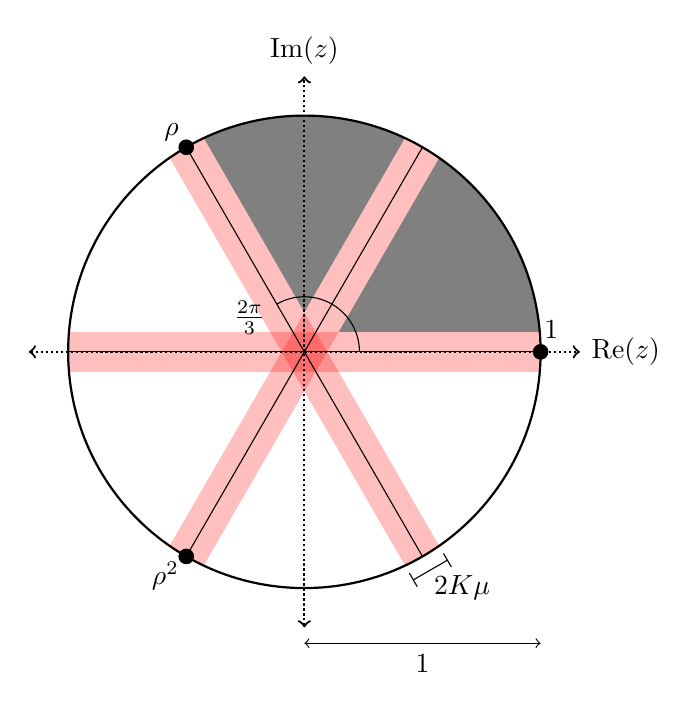
\begin{tikzpicture}	
	\filldraw[draw=none,color=gray] (0,0) -- (3,0) arc (0:120:3) -- (0,0);
		
	\begin{scope}[rotate=30]
		\draw[line width = 5mm, color=white] (0,-3) -- (0,3);
	\end{scope}
	\begin{scope}[rotate=90]
		\draw[line width = 5mm, color=white] (0,-3) -- (0,3);
	\end{scope}
	\begin{scope}[rotate=150]
		\draw[line width = 5mm, color=white] (0,-3) -- (0,3);
	\end{scope}
	
	\begin{scope}[rotate=30]
		\draw[line width = 5mm, color=Red,opacity=0.25] (0,-3) -- (0,3);
	\end{scope}
	\begin{scope}[rotate=90]
		\draw[line width = 5mm, color=Red,opacity=0.25] (0,-3) -- (0,3);
	\end{scope}
	\begin{scope}[rotate=150]
		\draw[line width = 5mm, color=Red,opacity=0.25] (0,-3) -- (0,3);
	\end{scope}
	
	\draw[thick,densely dotted,<->] (-3.5,0) -- (3.5,0);
	\draw[thick,densely dotted,<->] (0,-3.5) -- (0,3.5);
	
	\draw[<->] (0,-3.7) -- (3,-3.7);
	\draw (1.5,-3.6)  node[draw=none,fill=none,label=below:{$1$}]  {};
	
	\begin{scope}[rotate=-60]
		\draw[] (3.2,-0.25) -- (3.2,0.25);
		\draw (3.1,-0.25) -- (3.3,-0.25);
		\draw (3.1,0.25) -- (3.3,0.25);
	\end{scope}
	
	\foreach \x in {0,60,120,180,240,300} 
	{
		\draw[black] (0,0) -- (\x:3);
	}
	
	\draw[black,thick] (0,0) circle (3cm); 
	
	\draw (3.4,0)  node[draw=none,fill=none,label=right:{${\rm Re}(z)$}]  {};
	\draw (0,3.4)  node[draw=none,fill=none,label=above:{${\rm Im}(z)$}]  {};
	\draw (1.4,-3)  node[draw=none,fill=none,label=right:{$2K\mu$}]  (0) {};
	
	\draw (0.7,0) arc (0:120:0.7);
	\draw (120:0.5)  node[draw=none,fill=none,label=left:{$\frac{2\pi}{3}$}]  (0) {};
	
	\draw (0:2.8)  node[draw=none,fill=none,label=20:{$1$}]   {};
	\draw (120:2.8)  node[draw=none,fill=none,label=120:{$\rho$}]   {};
	\draw (240:2.8)  node[draw=none,fill=none,label=240:{$\rho^2$}]   {};
	
	\draw (0:3)  node[circle,inner sep=2,fill = black]   {};
	\draw (120:3)  node[circle,inner sep=2,fill = black]   {};
	\draw (240:3)  node[circle,inner sep=2,fill = black]   {};
	
\end{tikzpicture}
}
		\caption{An illustration of the position of $\innerp{\V{w}_i,\V{z}_j}$ for $p=3$. The pink stripes are the ones excluded in~\ref{it-between}(i); while the dark regions correspond to ~\ref{it-between}(ii).\label{fig:GBE}}
\end{figure}





\subsection{Structure of the inner graphs}
In this subsection, using isoperimetry and concentration of measure, we shall derive that the inner graphs $G[W], G[Z]$ are $K_{p+1}$-free graphs (Lemma~\ref{obs-samerotation}) with sublinear $p$-independence number (Lemma~\ref{lem-independenceGBEoneside}) and zero edge density (Lemma~\ref{lem-maxinsidedeg}), thus verifying~\ref{CBE:p-ind} and~\ref{CBE:sparse-inside}.


\begin{lemma}\label{obs-samerotation}
	Let $\V{w}_i,\V{w}_{j},\V{w}_{t}\in W$ span a triangle in $G$. If $\V{w}_i, \V{w}_{j}$ are an $h_i$- and $h_j$-rotation of $\V{w}_{t}$ respectively, then $\V{w}_i$ is an $(h_i-h_j)$-rotation of $\V{w}_{j}$ and $h_i\neq h_j$. 
	
	Consequently, $G[W]$ is $K_{ p+1}$-free. The same holds for $Z$.
\end{lemma}

\begin{proof}
	For any $m \in [p-1]$, we have
	\begin{equation}\label{eq-largenorm}
		|1-\rho^m|^2 = 2-2\cos \left(2\pi m/p\right) \geq 2-2\cos\left(2\pi/p\right) = 4\sin^2 \left(\pi/p\right) \geq \left(4/p\right)^2,
	\end{equation}
	as $\sin x\ge \frac{2x}{\pi}$ for all $x\in[0,\frac{\pi}{2}]$ by concavity.
	By~\ref{it-insideW}, there is $h\in [p-1]$ such that $\V{w}_i$ is an $h$-rotation of $\V{w}_j$. Recall that vertices of $G$, viewed as points in $\sS^{k-1}(\sC)$, all have modulus 1.
	So
	\begin{align*}
		|1-\rho^{h_i-h_j-h}| &= |\rho^h\V{w}_j-\rho^{h_i-h_j}\V{w}_j| \leq |\V{w}_i-\rho^h\V{w}_j| + |\V{w}_i-\rho^{h_i}\V{w}_t| + |\rho^{h_i}\V{w}_t-\rho^{h_i-h_j}\V{w}_j|\\
		&= |\V{w}_i-\rho^h\V{w}_j| + |\V{w}_i-\rho^{h_i}\V{w}_t| + |\V{w}_j-\rho^{h_j}\V{w}_t| \leq 3\sqrt{\mu},
	\end{align*}
	which together with~\eqref{eq-hierarchy} and~\eqref{eq-largenorm} implies $h=h_i-h_j$. Since $h\neq 0$, we have that $h_i \neq h_j$.
	
	Suppose that $\V{w}_0,\V{w}_1,\ldots,\V{w}_{ p}$ span a clique in $G[W]$. Then by~\ref{it-insideW} there are $h_1,\ldots,h_ p \in [p-1]$ such that $\V{w}_i$ is an $h_i$-rotation of $\V{w}_0$ for all $i \in [ p]$.
	By the Pigeonhole Principle, there are distinct $i,j \in [ p]$ such that $h_i=h_j$, contradicting the first part.
\end{proof}

\begin{lemma}\label{lem-independenceGBEoneside}
	Every set $X\subseteq W$ with $|X|\ge pe^{-\mu k/40}\cdot|W|$ contains a copy of $K_p$. In particular, $$\alpha_p(G)\le 2pe^{-\mu k/40}n.$$
\end{lemma}

For its proof, we need the following consequence of concentration of measure.


\begin{lemma}\label{lem-closebyrotations}
	Let $p\ge 2$ be an integer, $\nu\le \min\{\frac{16}{p^2},1\}$ and $A\subseteq \sS^{k-1}(\sC)$ with $\lambda(A)\ge pe^{-\nu k/32}$. Then there are distinct points $\V{a}_0,\ldots,\V{a}_{p-1}\in A$ such that, for all $h,m\in \sZ_p$,
	$$\bigabs{\rho^h\V{a}_h-\rho^m\V{a}_m}<\sqrt{\nu}.$$
\end{lemma}
\begin{proof}
	For all $h\in [p-1]$, define 
	$$
	A_h:=\left\{\V{a}\in A:~\forall \V{a}'\in A,~\bigabs{\V{a}+\rho^h\V{a}'}< 2-\nu/16 \right\}.
	$$
	Note that $\lambda(A_h)\le e^{-\nu k/32}$ as otherwise, the sets $A_h$ and $-\rho^hA$ violate Lemma~\ref{lem:cap-2set}. Therefore, $A\neq A_1\cup\cdots\cup A_{p-1}$, and we can pick a point $\V{a}_0\in A\setminus(A_1\cup\cdots\cup A_{p-1})$. 
	
	For all $h\in [p-1]$, since $\V{a}_0\notin A_h$, there exists a point $\V{a}_h\in A$
	with  $|\V{a}_0+\rho^h\V{a}_h|\ge 2-\nu/16$. We claim that $|\V{a}_0-\rho^h\V{a}_h|<\sqrt{\nu}/2$, for all $h\in \sZ_p$. The inequality is trivial for $h=0$. For $h\in [p-1]$, it follows from the parallelogram law:
	\begin{equation*}
		|\V{a}_0-\rho^h\V{a}_h|^2=  2(|\V{a}_0|^2+|\rho^h\V{a}_h|^2)-|\V{a}_0+\rho^h\V{a}_h|^2\le 4-(2-\nu/16)^2<\nu/4.
	\end{equation*}
	Thus, for all $h,m\in \sZ_p$, by the triangle inequality, we obtain
	\begin{equation}\label{eq-smallrotationdistance}
		|\rho^h\V{a}_h-\rho^m\V{a}_m|\le|\rho^h\V{a}_h-\V{a}_0|+|\V{a}_0-\rho^m\V{a}_m|<\sqrt{\nu}.
	\end{equation}

	We are left to show that all points $\V{a}_0,\ldots, \V{a}_{p-1}$ are distinct. Suppose to the contrary that for some distinct $h,m\in \sZ_p$, $\V{a}_h=\V{a}_m$. Then, as in~\eqref{eq-largenorm},
	\begin{equation*}
		|\rho^h\V{a}_h-\rho^m\V{a}_m|=|\rho^h-\rho^m|=|\rho^{h-m}-1|\ge  4/p\ge \sqrt{\nu},
	\end{equation*}   
	a contradiction to~\eqref{eq-smallrotationdistance}.
\end{proof}

We are now ready to prove Lemma~\ref{lem-independenceGBEoneside}.
\begin{proof}[Proof of Lemma~\ref{lem-independenceGBEoneside}]
Let $X\subseteq W$ with $|X|\ge pe^{-\mu k/40}\cdot|W|$
	and let $A:=\bigcup\{D_i:\V{w}_i\in X\}$; then $\lambda(A)=|X|/|W|\ge pe^{-\mu k/40}$. By Lemma~\ref{lem-closebyrotations}, there exist distinct $\V{a}_0,\ldots,\V{a}_{p-1}\in A$ such that $|\rho^h\V{a}_h-\rho^m\V{a}_m|\le \sqrt{4\mu/5}$ for all $h,m\in \sZ_p$. For each $h\in \sZ_p$, let $\V{x}_h\in X$ be the vertex lying in the same domain $D_i$ as $\V{a}_h$, i.e. $|\V{x}_h-\V{a}_h|\le \mu/4$. 
	
	Now, for distinct integers $h,m\in \sZ_p$, by triangle inequality and~\eqref{eq-hierarchy}, we get
	\begin{equation*}
		|\V{x}_h-\rho^{m-h}\V{x}_m|=|\rho^h\V{x}_h-\rho^m\V{x}_m|\le |\rho^h\V{x}_h-\rho^h\V{a}_h|+|\rho^h\V{a}_h-\rho^m\V{a}_m|+|\rho^m\V{a}_m-\rho^m\V{x}_m|\le\sqrt{\mu}.
	\end{equation*}
	Thus $\V{x}_h\V{x}_m\in E(G[W])$ and $\V{x}_0,\ldots,\V{x}_{p-1}$ induce a copy of $K_p$, finishing the proof.
\end{proof}

The fact that the inner graphs $G[W],G[Z]$ have zero edge density follows already from their being $K_{p+1}$-free and having sublinear $p$-independence number, as then their maximum degree is at most $\alpha_p(G[W])=e^{-\Theta(\sqrt{k})}n$ by Lemma~\ref{lem-independenceGBEoneside}. We can in fact give a tighter bound via a direct estimation. 
\begin{lemma}\label{lem-maxinsidedeg}
	The maximum degree of $G[W], G[Z]$ is at most $pe^{-k(1-\mu)^2}n\le e^{-k/2}n$. 
\end{lemma}

\begin{proof}
	By the construction of $G$, in particular~\ref{it-insideW} and that each domain $D_i$ has diameter at most $\mu/4$, we see that in $G[W]$ every vertex has degree $n(p-1)$ times the measure of a spherical cap whose points are within distance $d=\sqrt{\mu}\pm \mu/4$ from its centre. As the height of such a cap is precisely $d^2/2$, the conclusion follows from Lemma~\ref{lem:cap-UB}.
\end{proof}




\subsection{Angle decides cross density}
In this subsection, we verify~\ref{CBE:density}.
\begin{lemma}\label{lem-mindegree}
	Every vertex in $W$ has $(\frac{\ell}{p}\pm \frac{1}{\sqrt{K}}) n$  neighbours in $Z$, and vice versa.
\end{lemma}

\begin{proof}
For each point $\V{x}\in \sS^{k-1}(\sC)$, define sets
\begin{align*}
	J(\V{x})&:=\left\{\V{y}\in \sS^{k-1}(\sC): \bigabs{\iminnerp{\V{x}, \rho^h \V{y}}}>\textstyle{\left(K+\frac{1}{4}\right)}\mu, \text{ for all } h\in \sZ_p\right\},\text{ and }\\
	I(\V{x})&:=\left\{\V{y}\in J(\V{x}): \arg\innerp{\V{x},\V{y}}\in \left[1/\sqrt{K},~2\pi \ell/p-1/\sqrt{K}\right]\right\}.
\end{align*} 
We shall show that for each vertex $\V w\in W$, vertices whose domains intersect the associated set $I(\V w)$ are adjacent to $\V w$. That is, 
\begin{equation}\label{eq:Zw}
	Z_\V{w}:=\{\V{z}_j\in Z: D_j\cap I(\V{w})\neq \varnothing\}\subseteq N_G(\V w).
\end{equation}

We first bound the measure of this associated set.
\begin{claim}\label{lem-crossnbrs}
	For any $\V{x}\in \sS^{k-1}(\sC)$, we have $\lambda(I(\V{x}))\ge \frac{\ell}{p}-\frac{1}{\sqrt{K}}$.
\end{claim}
\begin{poc}
	Fix an arbitrary $\V{x}\in \sS^{k-1}(\sC)$. Define 
	$$L:=\left\{\V{y}\in \sS^{k-1}(\sC): |-\V{x}i-\V{y}|\le\sqrt{2}-K\mu\right\}.$$
	By Lemma~\ref{lem:cap-LB} (with $\delta=\eps K$), we see that $\lambda(L)\ge \frac{1}{2}-\sqrt{2}\eps K$. For each $y\in L$, using~\eqref{eq-hierarchy},
	%$L_1:=\{\V{y}\in \sS^{k-1}(\sC): |-i\V{x}-\V{y}|\le\sqrt{2}-K\mu\}$ and $L_2:=\{\V{y}\in \sS^{k-1}(\sC): |i\V{x}-\V{y}|\le\sqrt{2}-K\mu\}$. By Lemma~\ref{lem-CSCLB} (with $\delta=\eps K$), we have $\lambda(L_1), \lambda(L_2)\ge \frac{1}{2}-\sqrt{2}\eps K$. For any $j\in [2]$ and $y\in L_j$, we have
	\begin{equation*}
		2- 2\,\iminnerp{\V{x},\V{y}}=2-2\,\reinnerp{-\V{x}i,\V{y}}=|- \V{x}i-\V{y}|^2\le (\sqrt{2}-K\mu)^2<2-2\left(K+\tfrac{1}{4}\right)\mu,
	\end{equation*}
    and so  $\iminnerp{\V{x},\V{y}}>(K+\frac{1}{4})\mu$. Thus, by symmetry, the measure of the set
	$$
	\left\{\V{y}\in \sS^{k-1}(\sC): \bigabs{\iminnerp{\V{x},\V{y}}}\le\left(K+\tfrac{1}{4}\right)\mu\right\}$$
	is at most $1-2\lambda(L)\le 1-2\left(\frac{1}{2}-\sqrt{2}\eps K\right)=2\sqrt{2}\eps K$.
	Since $\innerp{\V{x},\rho^h\V{y}}=\innerp{\rho^{-h}\V{x},\V{y}}$, we can take the union bound of such sets over $\V{x}$, $\rho\V{x}$,$\ldots$, $\rho^{p-1}\V{x}$ to deduce that $\lambda(\overline{J(\V{x})})\le 2\sqrt{2}\eps Kp$, where $\overline{J(\V{x})}:=\sS^{k-1}(\sC)\setminus J(\V{x})$. Therefore, by~\eqref{eq-hierarchy}, we get
	\begin{equation*}
		\lambda(I(\V{x}))\ge\frac{1}{2\pi}\left(\frac{2\pi\ell}{p}-\frac{2}{\sqrt{K}}\right)-\lambda(\overline{J(\V{x})})\ge \frac{\ell}{p}-\frac{1}{\sqrt{K}}.
	\end{equation*}
\end{poc}


	Fix a vertex $\V{w}\in W$ and let $Z_{\V w}$ be as in~\eqref{eq:Zw}. As each domain $D_j$ has measure $\frac{1}{n}$, the above claim entails
	\begin{equation*}
		|Z_\V{w}|\ge n\sum_{\V{z}_{j}\in Z_\V{w}}\lambda(D_j\cap I(\V{w}))=n\cdot\lambda(I(\V{w}))\ge \left(\frac{\ell}{p}-\frac{1}{\sqrt{K}}\right)n.
	\end{equation*}  
    We are left to show $Z_{\V w}\subseteq N_G(\V w)$ and that the upper bound on the degrees can be obtained similarly.
	
	Fix a vertex $\V{z}_j\in Z_\V{w}$ and take a point $\V{z}^*\in D_j\cap I(\V{w})$. As $\V z_j,\V z^*\in D_j$, $|\V{z}^*-\V{z}_j|\le \mu/4$. For any $h\in \sZ_p$, using the triangle inequality, that $\V z^*\in I(\V{w})$, and the Cauchy–Schwarz inequality, we see that
	\begin{align*}
		|\im{\rho^h \innerp{\V{w},\V{z}_j}}|=|\iminnerp{\V{w},\rho^{-h}\V{z}_j}|&\ge |\iminnerp{\V{w},\rho^{-h}\V{z}^*}|-|\iminnerp{\V{w},\rho^{-h}\V{z}^*}-\iminnerp{\V{w},\rho^{-h}\V{z}_j}|\\
		&\ge (K+\tfrac{1}{4})\mu-|\innerp{\V{w},\rho^{-h}\V{z}^*}-\innerp{\V{w},\rho^{-h}\V{z}_j}|\\
		&\ge(K+\tfrac{1}{4})\mu-|\V{w}|\cdot|\rho^{-h}\V{z}^*-\rho^{-h}\V{z}_{j}|\\
		&=(K+\tfrac{1}{4})\mu-|\V{z}^*-\V{z}_{j}|\ge K\mu,
	\end{align*}  
	verifying~\ref{it-between}(i). 
	
	For~\ref{it-between}(ii), let $x:=\innerp{\V{w},\V{z}_j}$ and $y:=\innerp{\V{w},\V{z}^*}$. Then as above we have $|y|\ge |\iminnerp{\V{w},\V{z}^*}|\ge (K+\frac{1}{4})\mu$, $|x-y|\le |\V w||\V z^*-\V z_j|\le \mu/4$ and so $|x|\ge |y|-|x-y|\ge K\mu$.
	Consider the triangle in the complex plane with vertices $0,x,y$ and let $\alpha$ be its angle at $0$. Then the law of cosines implies that
	$$\cos\alpha=\frac{|x|^2+|y|^2-|x-y|^2}{2|x||y|}\ge\frac{(1-\frac{1}{8K})(|x|^2+|y|^2)}{2|x||y|}\ge 1-\frac{1}{8K}.$$
	As $\cos \theta\le 1-\frac{\theta^2}{4}$ when $\theta\in(0,1)$, we get $|\arg\innerp{\V{w},\V{z}_j} - \arg\innerp{\V{w},\V{z}^*}|=\alpha\le 1/\sqrt{2K}$. Therefore $\arg\innerp{\V{w},\V{z}_j}\in [0,2\pi\ell/p]$ as $\V z^*\in I(\V w)$, implying~\ref{it-between}(ii).
	
	We omit the proof of the upper bound on degrees since it is very similar but easier, noting that the upper bound corresponding to Claim~\ref{lem-crossnbrs} is clear as the set of $\V{y} \in \sS^{k-1}(\mathbb{C})$ with $\arg\innerp{\V{x},\V{y}} \in [s,t]$ trivially has measure at most $\frac{t-s}{2\pi}$.
\end{proof}


 
\subsection{Clique number of $G$}
Finally, we verify~\ref{CBE:clique}. 
We will need the following lemma. 

\begin{lemma}\label{lem-farpairs}
	Let $U$ be a subset of $W$ or $Z$ such that $G[U]$ is a clique. Then there exists a pair of vertices $\V{u},\V{u}'\in U$ such that $\V{u}$ is an $h$-rotation of $\V{u}'$ with $\min\{|U|-1, \floor{p/2}\}\le h\le \floor{p/2}$.
\end{lemma}
\begin{proof}
	Note that the upper bound is trivial, as in every pair of adjacent vertices, taking the smaller angle we see that one is an $h$-rotation of the other for some $h\le \floor{p/2}$. For the lower bound, set $u:=|U|$. We will prove the case when $u-1\le \floor{p/2}$. The other case can be reduced to this case by taking a subset of $U$ of size $\floor{p/2}+1$. 
	
	Fix a vertex $\V{u}_0\in U$. By~\ref{it-insideW},  every vertex $\V{u}\in U\setminus\{\V{u}_0\}$ is an $h$-rotation of $\V{u}_0$, for some $h\in[p-1]$. We may assume that $h\in \{-u+2,\ldots,u-2\}\setminus\{0\}$, for otherwise, $\V{u}_0,\V{u}$ is the pair we seek. Pair up all elements in $\{-u+2,\ldots,u-2\}\setminus\{0\}$ such that their difference is $u-1$, that is, partition it into pairs $\{-u+1+j,j\}$, for all $j\in [u-2]$. We say a vertex in $U\setminus\{\V{u}_0\}$ \emph{belongs to the $j$-th pair} if it is either a $(-u+1+j)$-rotation or a $j$-rotation of $\V{u}_0$. By the Pigeonhole Principle, there exists a pair of vertices $\V{u},\V{u}'\in U\setminus\{\V{u}_0\}$ that form the $j$-th pair for some $j\in[u-2]$. By Lemma~\ref{obs-samerotation}, they are not the same rotation of $\V{u}_0$. Therefore, without loss of generality, we can assume that $\V{u}$ is a $j$-rotation of $\V{u}_0$ and $\V{u}'$ is a $(-u+1+j)$-rotation of $\V{u}_0$. Thus, by Lemma~\ref{obs-samerotation}, $\V{u}$ is a $(u-1)$-rotation of $\V{u}'$.
\end{proof}


Take $\ell\le p/2$. Suppose to the contrary that $G$ contains a copy of $K_{p+\ell+1}$ on vertex set $X\cup Y$, with, say, $X\subseteq W$, $Y\subseteq Z$ and $|X|\ge |Y|$.
So $\frac{p}{2} < |X| \leq p$ (since $X$ is $K_{p+1}$-free) and hence $|Y| \geq \ell+1$.
Let $\V{x}_0 \in X$ be arbitrary, set
$$
A := \{h \in \mathbb{Z}_p: X \text{ contains an } h\text{-rotation of }\V{x}_0\}\quad\text{and}\quad B := \{\rho^h: h \in A\} \subseteq \{z \in \mathbb{C} : |z|=1\}.
$$
If the closed convex hull of $B$ fails to contain $0$, then $B$ is contained in an open half-plane of $\mathbb{C}$ bounded by a line passing through $0$, so we have $|X|=|B| \leq \frac{p}{2}$, a contradiction.
Thus $0$ lies in the closed convex hull of $B$. Consequently, by Carath\'eodory's theorem, there are $h_1,h_2,h_3 \in A$ such that $0$ is in the closed triangle with vertices $\rho^{h_1},\rho^{h_2},\rho^{h_3}$.
In other words, there are reals $\lambda_1,\lambda_2,\lambda_3 \in [0,1]$ such that $\lambda_1+\lambda_2+\lambda_3 =1$ and $\lambda_1\rho^{h_1}+\lambda_2\rho^{h_2}+\lambda_3\rho^{h_3}=0$.
Pick $\V{x}_1,\V{x}_2,\V{x}_3 \in X$ such that $|\V{x}_i-\rho^{h_i}\V{x}_0| \leq \sqrt{\mu}$ for all $i \in [3]$.
By the triangle inequality
$$
\V{x} := \lambda_1\V{x}_1+\lambda_2\V{x}_2+\lambda_3\V{x}_3 = \lambda_1(\V{x}_1-\rho^{h_1}\V{x}_0)+\lambda_2(\V{x}_2-\rho^{h_2}\V{x}_0)+\lambda_3(\V{x}_3-\rho^{h_3}\V{x}_0) 
$$
satisfies $|\V{x}| \leq \sqrt{\mu}$.
By Lemma~\ref{lem-farpairs}, there exist a pair of vertices $\V{y},\V{y}' \in Y$ and an integer $m$ such that $\ell \leq m \leq \frac{p}{2}$ and $|\V{y}-\rho^m\V{y}'| \leq \sqrt{\mu}$. Now,
\begin{equation}\label{eq-xyy'}
\iminnerp{\V{x},\V{y}-\rho^m\V{y}'} \leq |\innerp{\V{x},\V{y}-\rho^m\V{y}'}| \leq |\V{x}||\V{y}-\rho^m\V{y}'| \leq \mu.
\end{equation}
 On the other hand,~\ref{it-between}(ii) implies that $0 \leq \arg\innerp{\V{x}_i,\V{y}}, \arg\innerp{\V{x}_i,\V{y}'} \leq \frac{2\pi\ell}{p}$. So
 $$
 0 \leq \arg(-\rho^{-m}\innerp{\V{x}_i,\V{y}'}) \leq 2\pi\left(\frac{\ell}{p}+\frac{p/2-m}{p}\right) \leq \pi
 $$
 since $\ell \leq m$.
 So the imaginary parts of $\innerp{\V{x}_i,\V{y}},-\rho^{-m}\innerp{\V{x}_i,\V{y}'}$ are positive, and
 \ref{it-between}(i) yields
$$
\iminnerp{\V{x}_i,\V{y}}, \im{-\rho^{-m}\innerp{\V{x}_i,\V{y}'}} \geq K\mu\quad\text{for all }i \in [3], 
$$
whence $\iminnerp{\V{x},\V{y}-\rho^m\V{y}'} \geq 2K\mu$.
This contradiction to~(\ref{eq-xyy'}) concludes the proof of~\ref{CBE:clique}.

\begin{thebibliography}{99}
\bibitem{BL-1}
J.~Balogh and J.~Lenz,
\newblock On the {R}amsey-{T}ur\'an numbers of graphs and hypergraphs,
\newblock {\em Israel J. Math.}, 194~(1), (2013), 45--68.

\bibitem{EHSSSz}
P.~Erd\H os, A.~Hajnal, M.~Simonovits, V.~T.~S\'os and E.~Szemer\'edi,
\newblock Tur\'an-Ramsey theorems and \text{$K_p$-independence} numbers,
\newblock{\em Combinatorics, Probability and Computing}, 3, (1994), 297-325.

\bibitem{EHSSz}
P.~Erd\H os, A.~Hajnal, V.~T.~S\'os and E.~Szemer\'edi,
\newblock More results on Ramsey-Tur\'an type problems,
\newblock {\em Combinatorica}, 3(1), (1983), 69--81.

\bibitem{FS}
U.~Feige and G.~Schechtman,
\newblock On the optimality of the random hyperplane rounding technique for MAX CUT,
\newblock {\em Ramdom Structures Algorithms}, 20, (2002), 403--440.

\bibitem{Schmidt}
E.~Schmidt, 
\newblock Die Brunn-Minkowski Ungleichung und ihr Spiegelbild sowie die isoperimetrische Eigenschaft der Kugel in der euklidischen und nichteuklidischen
\newblock {\em Geometrie I}, Math Nachrichten, Berlin 1, (1948), 81--157.

\bibitem{Tkocz}
T.~Tkocz,
\newblock An upper bound for spherical caps,
\newblock {\em Amer. Math. Monthly}, 119 (7), (2012), 606--607.

\end{thebibliography}
\end{document}
